% Options for packages loaded elsewhere
\PassOptionsToPackage{unicode}{hyperref}
\PassOptionsToPackage{hyphens}{url}
\documentclass[
]{article}
\usepackage{xcolor}
\usepackage[margin=1in]{geometry}
\usepackage{amsmath,amssymb}
\setcounter{secnumdepth}{-\maxdimen} % remove section numbering
\usepackage{iftex}
\ifPDFTeX
  \usepackage[T1]{fontenc}
  \usepackage[utf8]{inputenc}
  \usepackage{textcomp} % provide euro and other symbols
\else % if luatex or xetex
  \usepackage{unicode-math} % this also loads fontspec
  \defaultfontfeatures{Scale=MatchLowercase}
  \defaultfontfeatures[\rmfamily]{Ligatures=TeX,Scale=1}
\fi
\usepackage{lmodern}
\ifPDFTeX\else
  % xetex/luatex font selection
\fi
% Use upquote if available, for straight quotes in verbatim environments
\IfFileExists{upquote.sty}{\usepackage{upquote}}{}
\IfFileExists{microtype.sty}{% use microtype if available
  \usepackage[]{microtype}
  \UseMicrotypeSet[protrusion]{basicmath} % disable protrusion for tt fonts
}{}
\makeatletter
\@ifundefined{KOMAClassName}{% if non-KOMA class
  \IfFileExists{parskip.sty}{%
    \usepackage{parskip}
  }{% else
    \setlength{\parindent}{0pt}
    \setlength{\parskip}{6pt plus 2pt minus 1pt}}
}{% if KOMA class
  \KOMAoptions{parskip=half}}
\makeatother
\usepackage{color}
\usepackage{fancyvrb}
\newcommand{\VerbBar}{|}
\newcommand{\VERB}{\Verb[commandchars=\\\{\}]}
\DefineVerbatimEnvironment{Highlighting}{Verbatim}{commandchars=\\\{\}}
% Add ',fontsize=\small' for more characters per line
\usepackage{framed}
\definecolor{shadecolor}{RGB}{248,248,248}
\newenvironment{Shaded}{\begin{snugshade}}{\end{snugshade}}
\newcommand{\AlertTok}[1]{\textcolor[rgb]{0.94,0.16,0.16}{#1}}
\newcommand{\AnnotationTok}[1]{\textcolor[rgb]{0.56,0.35,0.01}{\textbf{\textit{#1}}}}
\newcommand{\AttributeTok}[1]{\textcolor[rgb]{0.13,0.29,0.53}{#1}}
\newcommand{\BaseNTok}[1]{\textcolor[rgb]{0.00,0.00,0.81}{#1}}
\newcommand{\BuiltInTok}[1]{#1}
\newcommand{\CharTok}[1]{\textcolor[rgb]{0.31,0.60,0.02}{#1}}
\newcommand{\CommentTok}[1]{\textcolor[rgb]{0.56,0.35,0.01}{\textit{#1}}}
\newcommand{\CommentVarTok}[1]{\textcolor[rgb]{0.56,0.35,0.01}{\textbf{\textit{#1}}}}
\newcommand{\ConstantTok}[1]{\textcolor[rgb]{0.56,0.35,0.01}{#1}}
\newcommand{\ControlFlowTok}[1]{\textcolor[rgb]{0.13,0.29,0.53}{\textbf{#1}}}
\newcommand{\DataTypeTok}[1]{\textcolor[rgb]{0.13,0.29,0.53}{#1}}
\newcommand{\DecValTok}[1]{\textcolor[rgb]{0.00,0.00,0.81}{#1}}
\newcommand{\DocumentationTok}[1]{\textcolor[rgb]{0.56,0.35,0.01}{\textbf{\textit{#1}}}}
\newcommand{\ErrorTok}[1]{\textcolor[rgb]{0.64,0.00,0.00}{\textbf{#1}}}
\newcommand{\ExtensionTok}[1]{#1}
\newcommand{\FloatTok}[1]{\textcolor[rgb]{0.00,0.00,0.81}{#1}}
\newcommand{\FunctionTok}[1]{\textcolor[rgb]{0.13,0.29,0.53}{\textbf{#1}}}
\newcommand{\ImportTok}[1]{#1}
\newcommand{\InformationTok}[1]{\textcolor[rgb]{0.56,0.35,0.01}{\textbf{\textit{#1}}}}
\newcommand{\KeywordTok}[1]{\textcolor[rgb]{0.13,0.29,0.53}{\textbf{#1}}}
\newcommand{\NormalTok}[1]{#1}
\newcommand{\OperatorTok}[1]{\textcolor[rgb]{0.81,0.36,0.00}{\textbf{#1}}}
\newcommand{\OtherTok}[1]{\textcolor[rgb]{0.56,0.35,0.01}{#1}}
\newcommand{\PreprocessorTok}[1]{\textcolor[rgb]{0.56,0.35,0.01}{\textit{#1}}}
\newcommand{\RegionMarkerTok}[1]{#1}
\newcommand{\SpecialCharTok}[1]{\textcolor[rgb]{0.81,0.36,0.00}{\textbf{#1}}}
\newcommand{\SpecialStringTok}[1]{\textcolor[rgb]{0.31,0.60,0.02}{#1}}
\newcommand{\StringTok}[1]{\textcolor[rgb]{0.31,0.60,0.02}{#1}}
\newcommand{\VariableTok}[1]{\textcolor[rgb]{0.00,0.00,0.00}{#1}}
\newcommand{\VerbatimStringTok}[1]{\textcolor[rgb]{0.31,0.60,0.02}{#1}}
\newcommand{\WarningTok}[1]{\textcolor[rgb]{0.56,0.35,0.01}{\textbf{\textit{#1}}}}
\usepackage{graphicx}
\makeatletter
\newsavebox\pandoc@box
\newcommand*\pandocbounded[1]{% scales image to fit in text height/width
  \sbox\pandoc@box{#1}%
  \Gscale@div\@tempa{\textheight}{\dimexpr\ht\pandoc@box+\dp\pandoc@box\relax}%
  \Gscale@div\@tempb{\linewidth}{\wd\pandoc@box}%
  \ifdim\@tempb\p@<\@tempa\p@\let\@tempa\@tempb\fi% select the smaller of both
  \ifdim\@tempa\p@<\p@\scalebox{\@tempa}{\usebox\pandoc@box}%
  \else\usebox{\pandoc@box}%
  \fi%
}
% Set default figure placement to htbp
\def\fps@figure{htbp}
\makeatother
\setlength{\emergencystretch}{3em} % prevent overfull lines
\providecommand{\tightlist}{%
  \setlength{\itemsep}{0pt}\setlength{\parskip}{0pt}}
\usepackage{bookmark}
\IfFileExists{xurl.sty}{\usepackage{xurl}}{} % add URL line breaks if available
\urlstyle{same}
\hypersetup{
  pdftitle={Additional simulation results},
  hidelinks,
  pdfcreator={LaTeX via pandoc}}

\title{Additional simulation results}
\author{}
\date{\vspace{-2.5em}}

\begin{document}
\maketitle

\begin{Shaded}
\begin{Highlighting}[]
\FunctionTok{source}\NormalTok{(}\StringTok{"process{-}simulation{-}results.R"}\NormalTok{)}
\end{Highlighting}
\end{Shaded}

\begin{verbatim}
## -- Attaching core tidyverse packages ------------------------ tidyverse 2.0.0 --
## v dplyr     1.1.4     v readr     2.1.5
## v forcats   1.0.0     v stringr   1.5.1
## v ggplot2   3.5.2     v tibble    3.3.0
## v lubridate 1.9.3     v tidyr     1.3.1
## v purrr     1.0.4     
## -- Conflicts ------------------------------------------ tidyverse_conflicts() --
## x dplyr::filter() masks stats::filter()
## x dplyr::lag()    masks stats::lag()
## i Use the conflicted package (<http://conflicted.r-lib.org/>) to force all conflicts to become errors
\end{verbatim}

\begin{Shaded}
\begin{Highlighting}[]
\NormalTok{mu\_graph\_res\_main}\SpecialCharTok{$}\NormalTok{method }\OtherTok{=} \FunctionTok{fct}\NormalTok{(mu\_graph\_res\_main}\SpecialCharTok{$}\NormalTok{method, }\AttributeTok{levels =} \FunctionTok{c}\NormalTok{(}\StringTok{"Beta"}\NormalTok{,}\StringTok{"CHE{-}ISCW"}\NormalTok{,}\StringTok{"PET/PEESE"}\NormalTok{))}
\NormalTok{mu\_graph\_res\_ci\_main}\SpecialCharTok{$}\NormalTok{method }\OtherTok{=} \FunctionTok{fct}\NormalTok{(mu\_graph\_res\_ci\_main}\SpecialCharTok{$}\NormalTok{method, }\AttributeTok{levels =} \FunctionTok{c}\NormalTok{(}\StringTok{"Beta"}\NormalTok{,}\StringTok{"CHE{-}ISCW"}\NormalTok{,}\StringTok{"PET/PEESE"}\NormalTok{))}

\NormalTok{mu\_graph\_res\_miss}\SpecialCharTok{$}\NormalTok{method }\OtherTok{=} \FunctionTok{fct}\NormalTok{(mu\_graph\_res\_miss}\SpecialCharTok{$}\NormalTok{method, }\AttributeTok{levels =} \FunctionTok{c}\NormalTok{(}\StringTok{"Beta"}\NormalTok{,}\StringTok{"3PSM"}\NormalTok{,}\StringTok{"4PSM"}\NormalTok{))}
\NormalTok{mu\_graph\_res\_ci\_miss}\SpecialCharTok{$}\NormalTok{method }\OtherTok{=} \FunctionTok{fct}\NormalTok{(mu\_graph\_res\_ci\_miss}\SpecialCharTok{$}\NormalTok{method, }\AttributeTok{levels =} \FunctionTok{c}\NormalTok{(}\StringTok{"Beta"}\NormalTok{,}\StringTok{"3PSM"}\NormalTok{,}\StringTok{"4PSM"}\NormalTok{))}
\end{Highlighting}
\end{Shaded}

\section{Beta-Function Selection Model Compared to CHE-ISCW and
PET/PEESE}\label{beta-function-selection-model-compared-to-che-iscw-and-petpeese}

\subsection{\texorpdfstring{Additional simulation results for methods of
estimating the average effect size
\((\mu)\)}{Additional simulation results for methods of estimating the average effect size (\textbackslash mu)}}\label{mu-simulation-results-main}

\begin{Shaded}
\begin{Highlighting}[]
\NormalTok{mu\_graph\_res\_main }\SpecialCharTok{\%\textgreater{}\%}
  \FunctionTok{filter}\NormalTok{(model\_estimator }\SpecialCharTok{\%in\%} \FunctionTok{c}\NormalTok{(}\StringTok{"beta\_CML"}\NormalTok{)) }\SpecialCharTok{\%\textgreater{}\%}
  \FunctionTok{group\_by}\NormalTok{(mean\_smd, tau, selection\_strength, method) }\SpecialCharTok{\%\textgreater{}\%}
  \FunctionTok{summarize}\NormalTok{(}
    \AttributeTok{min =} \FunctionTok{min}\NormalTok{(convergence),}
    \AttributeTok{Q10 =} \FunctionTok{quantile}\NormalTok{(convergence, }\FloatTok{0.1}\NormalTok{),}
    \AttributeTok{median =} \FunctionTok{median}\NormalTok{(convergence),}
    \AttributeTok{Q90 =} \FunctionTok{quantile}\NormalTok{(convergence, }\FloatTok{0.9}\NormalTok{),}
    \AttributeTok{max =} \FunctionTok{max}\NormalTok{(convergence),}
    \AttributeTok{.groups =} \StringTok{"drop"}
\NormalTok{  ) }\SpecialCharTok{\%\textgreater{}\%}
\FunctionTok{ggplot}\NormalTok{() }\SpecialCharTok{+} 
  \FunctionTok{aes}\NormalTok{(}\AttributeTok{x =}\NormalTok{ selection\_strength, }\AttributeTok{y =}\NormalTok{ median, }\AttributeTok{ymin =}\NormalTok{ min, }\AttributeTok{max =}\NormalTok{ max, }\AttributeTok{color =}\NormalTok{ method, }\AttributeTok{fill =}\NormalTok{ method) }\SpecialCharTok{+}
  \FunctionTok{geom\_pointrange}\NormalTok{(}
    \AttributeTok{position =} \FunctionTok{position\_dodge}\NormalTok{(}\AttributeTok{width =} \FloatTok{0.5}\NormalTok{)}
\NormalTok{  ) }\SpecialCharTok{+} 
  \FunctionTok{geom\_linerange}\NormalTok{(}
    \FunctionTok{aes}\NormalTok{(}\AttributeTok{ymin =}\NormalTok{ Q10, }\AttributeTok{ymax =}\NormalTok{ Q90),}
    \AttributeTok{position =} \FunctionTok{position\_dodge}\NormalTok{(}\AttributeTok{width =} \FloatTok{0.5}\NormalTok{),}
    \AttributeTok{linewidth =} \FloatTok{1.2}
\NormalTok{  ) }\SpecialCharTok{+} 
  \FunctionTok{scale\_color\_brewer}\NormalTok{(}\AttributeTok{palette =} \StringTok{"Dark2"}\NormalTok{) }\SpecialCharTok{+}
  \FunctionTok{scale\_fill\_brewer}\NormalTok{(}\AttributeTok{palette =} \StringTok{"Dark2"}\NormalTok{) }\SpecialCharTok{+}
  \FunctionTok{scale\_x\_discrete}\NormalTok{(}\AttributeTok{labels =} \ControlFlowTok{function}\NormalTok{(x) stringr}\SpecialCharTok{::}\FunctionTok{str\_wrap}\NormalTok{(x, }\AttributeTok{width =} \DecValTok{3}\NormalTok{)) }\SpecialCharTok{+}
  \FunctionTok{expand\_limits}\NormalTok{(}\AttributeTok{y =} \FloatTok{0.99}\NormalTok{) }\SpecialCharTok{+} 
  \FunctionTok{facet\_grid}\NormalTok{(}
\NormalTok{    tau }\SpecialCharTok{\textasciitilde{}}\NormalTok{ mean\_smd, }
    \AttributeTok{labeller =} \FunctionTok{label\_bquote}\NormalTok{(}
      \AttributeTok{rows =}\NormalTok{ tau }\SpecialCharTok{==}\NormalTok{ .(tau),}
      \AttributeTok{cols =}\NormalTok{ mu }\SpecialCharTok{==}\NormalTok{ .(mean\_smd)}
\NormalTok{    ),}
    \AttributeTok{scales =} \StringTok{"free\_y"}
\NormalTok{  ) }\SpecialCharTok{+}
  \FunctionTok{labs}\NormalTok{(}
    \AttributeTok{x =} \StringTok{"Selection probability"}\NormalTok{, }
    \AttributeTok{y =} \StringTok{"Convergence rate"}\NormalTok{, }
    \AttributeTok{color =} \StringTok{"Method"}\NormalTok{,}
    \AttributeTok{fill =} \StringTok{"Method"}
\NormalTok{  ) }\SpecialCharTok{+} 
  \FunctionTok{theme\_bw}\NormalTok{() }\SpecialCharTok{+}
  \FunctionTok{theme}\NormalTok{(}\AttributeTok{legend.position =} \StringTok{"top"}\NormalTok{)}
\end{Highlighting}
\end{Shaded}

\begin{sidewaysfigure}
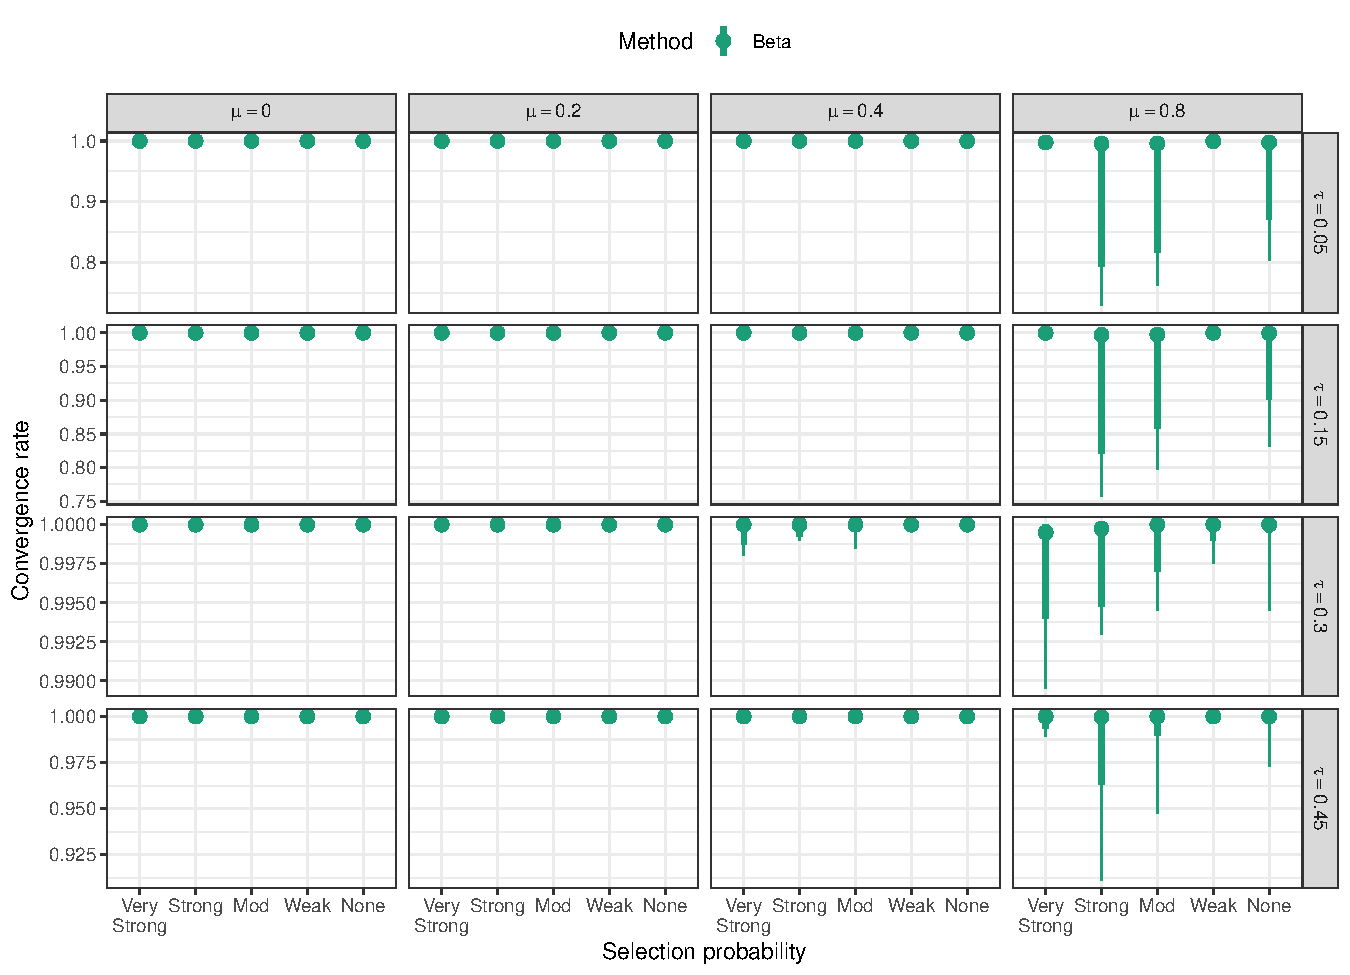
\includegraphics{appendix-simulation-results_files/figure-latex/convergence-rates-main-1} \caption{Convergence rates of the beta-function selection model by selection probability, average SMD, and between-study heterogeneity. Points correspond to median convergence rates; thin lines correspond to range of convergence rates; thick lines correspond to inter-decile range.}\label{fig:convergence-rates-main}
\end{sidewaysfigure}

\begin{Shaded}
\begin{Highlighting}[]
\FunctionTok{RMSE\_comparison\_plot}\NormalTok{(mu\_wide\_res\_main, }\StringTok{"Beta"}\NormalTok{,}\StringTok{"CHE{-}ISCW"}\NormalTok{)}
\end{Highlighting}
\end{Shaded}

\begin{sidewaysfigure}
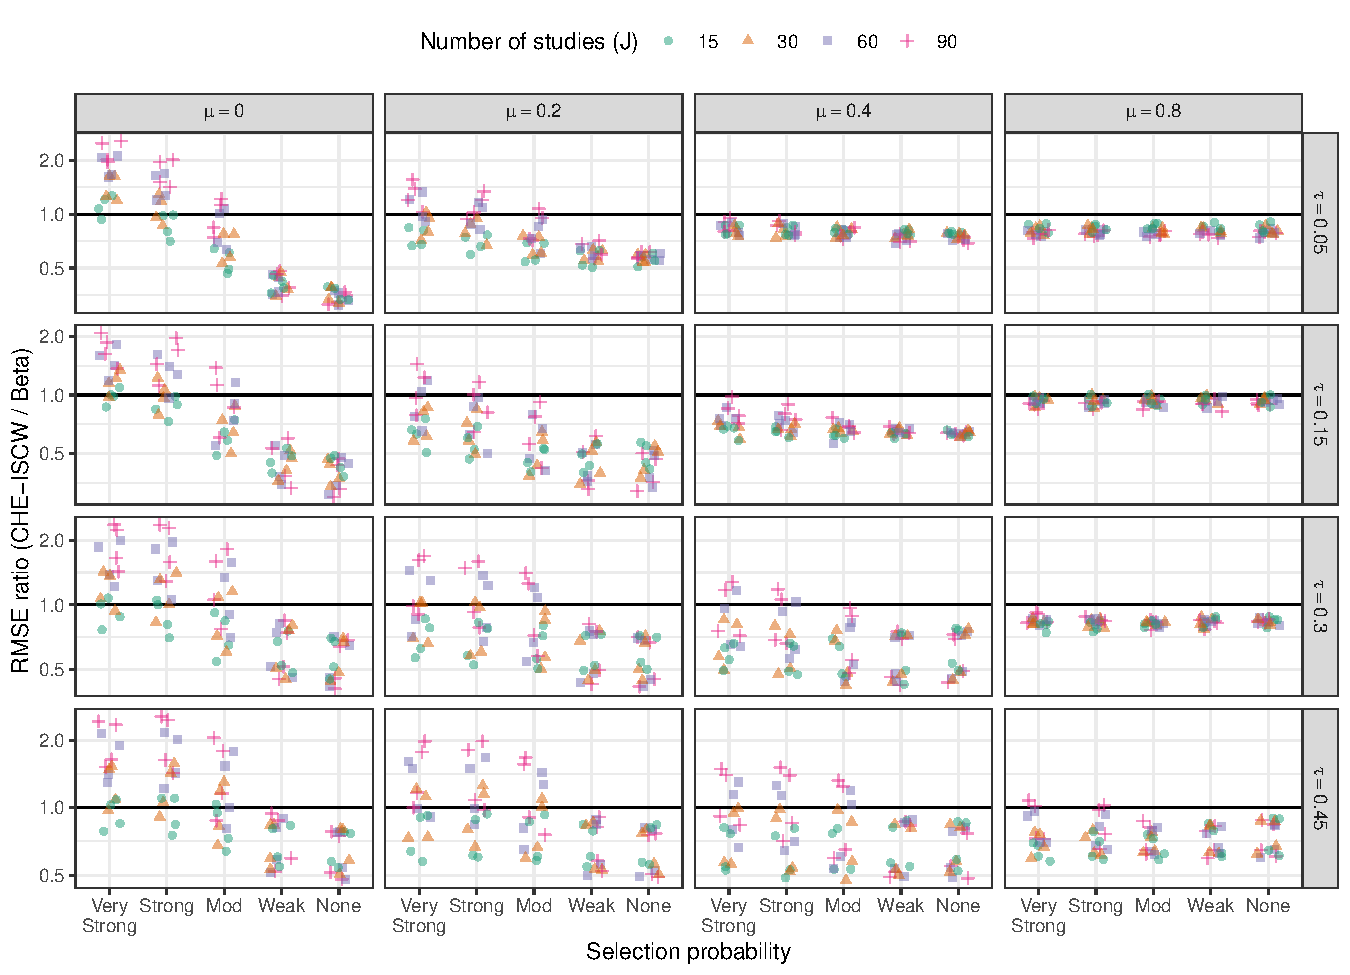
\includegraphics{appendix-simulation-results_files/figure-latex/rmse-CHE-Beta-main-1} \caption{Ratio of root mean-squared error for CHE-ISCW estimator to root mean-squared error of CML estimator by selection probability, number of studies, average SMD, and between-study heterogeneity}\label{fig:rmse-CHE-Beta-main}
\end{sidewaysfigure}

\begin{Shaded}
\begin{Highlighting}[]
\FunctionTok{RMSE\_comparison\_plot}\NormalTok{(mu\_wide\_res\_main, }\StringTok{"Beta"}\NormalTok{,}\StringTok{"PET/PEESE"}\NormalTok{)}
\end{Highlighting}
\end{Shaded}

\begin{sidewaysfigure}
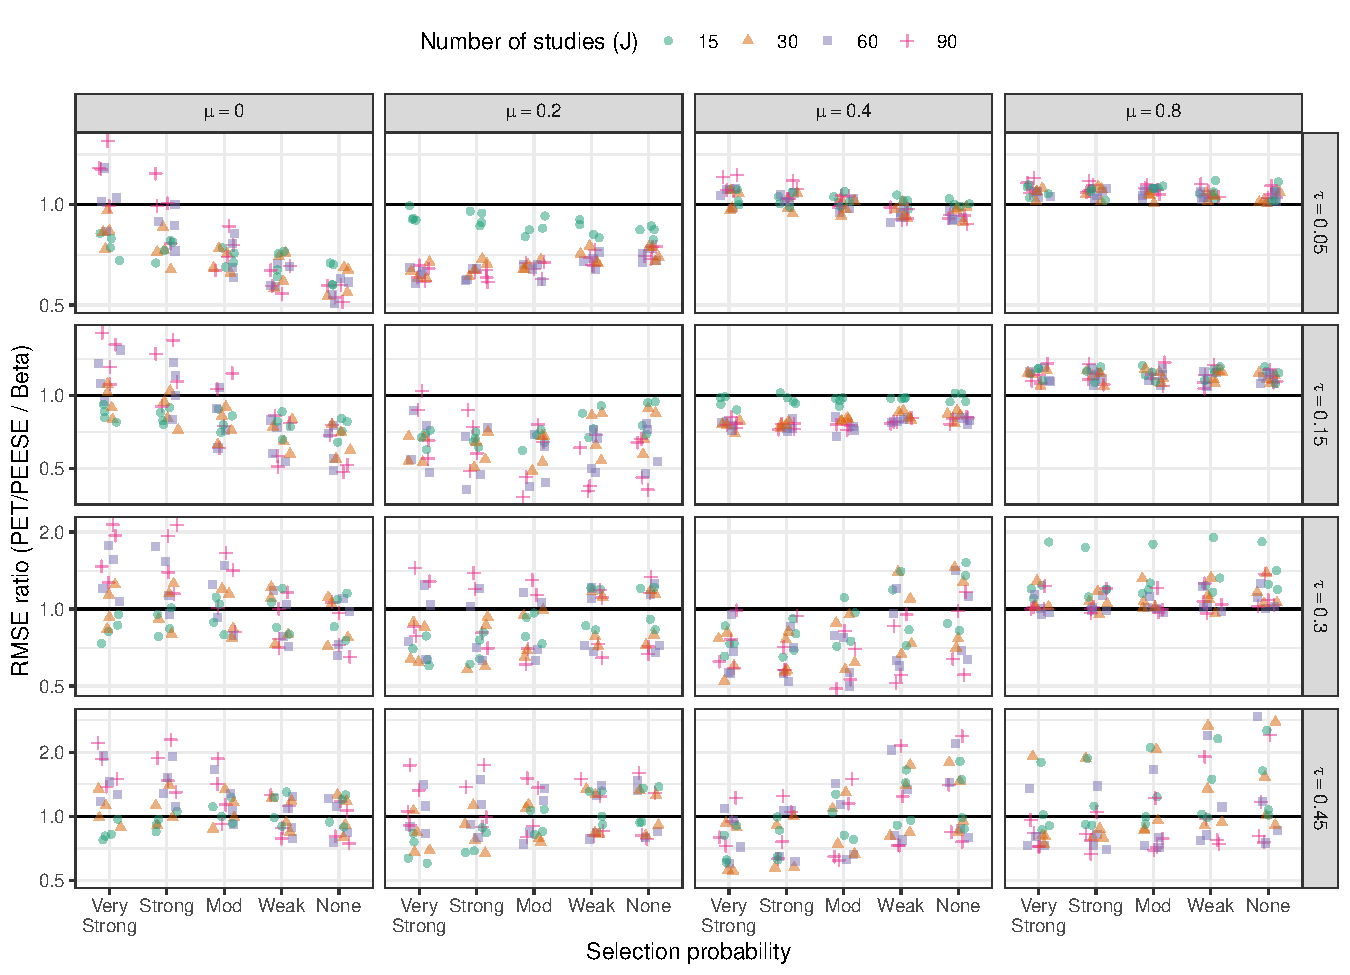
\includegraphics{appendix-simulation-results_files/figure-latex/rmse-PET-Beta-main-1} \caption{Ratio of root mean-squared error for PET/PEESE estimator to root mean-squared error of CML estimator by selection probability, number of studies, average SMD, and between-study heterogeneity}\label{fig:rmse-PET-Beta-main}
\end{sidewaysfigure}

\begin{Shaded}
\begin{Highlighting}[]
\NormalTok{mu\_graph\_res\_ci\_main }\SpecialCharTok{\%\textgreater{}\%}
  \FunctionTok{filter}\NormalTok{(}
\NormalTok{    CI\_type }\SpecialCharTok{\%in\%} \FunctionTok{c}\NormalTok{(}\StringTok{"large{-}sample"}\NormalTok{)}
\NormalTok{  ) }\SpecialCharTok{\%\textgreater{}\%}
  \FunctionTok{ggplot}\NormalTok{(}\FunctionTok{aes}\NormalTok{(}\AttributeTok{x =}\NormalTok{ J, }\AttributeTok{y =}\NormalTok{ coverage, }\AttributeTok{color =}\NormalTok{ method, }\AttributeTok{fill =}\NormalTok{ method)) }\SpecialCharTok{+}
  \FunctionTok{geom\_boxplot}\NormalTok{(}\AttributeTok{alpha =}\NormalTok{ .}\DecValTok{5}\NormalTok{, }\AttributeTok{coef =} \ConstantTok{Inf}\NormalTok{) }\SpecialCharTok{+}
  \FunctionTok{geom\_hline}\NormalTok{(}\AttributeTok{yintercept =} \FloatTok{0.95}\NormalTok{, }\AttributeTok{linetype =} \StringTok{"dashed"}\NormalTok{) }\SpecialCharTok{+}
  \FunctionTok{scale\_y\_continuous}\NormalTok{(}\AttributeTok{limits =} \FunctionTok{c}\NormalTok{(}\ConstantTok{NA}\NormalTok{, }\DecValTok{1}\NormalTok{), }\AttributeTok{expand =} \FunctionTok{expansion}\NormalTok{(}\DecValTok{0}\NormalTok{,}\DecValTok{0}\NormalTok{)) }\SpecialCharTok{+} 
  \FunctionTok{scale\_color\_brewer}\NormalTok{(}\AttributeTok{palette =} \StringTok{"Dark2"}\NormalTok{) }\SpecialCharTok{+}
  \FunctionTok{scale\_fill\_brewer}\NormalTok{(}\AttributeTok{palette =} \StringTok{"Dark2"}\NormalTok{) }\SpecialCharTok{+}
  \FunctionTok{facet\_grid}\NormalTok{(}
\NormalTok{    tau }\SpecialCharTok{\textasciitilde{}}\NormalTok{ mean\_smd, }
    \AttributeTok{labeller =} \FunctionTok{label\_bquote}\NormalTok{(}
      \AttributeTok{rows =}\NormalTok{ tau }\SpecialCharTok{==}\NormalTok{ .(tau),}
      \AttributeTok{cols =}\NormalTok{ mu }\SpecialCharTok{==}\NormalTok{ .(mean\_smd)}
\NormalTok{    ),}
    \AttributeTok{scales =} \StringTok{"free\_y"}
\NormalTok{  ) }\SpecialCharTok{+}
  \FunctionTok{labs}\NormalTok{(}
    \AttributeTok{x =} \StringTok{"Number of studies (J)"}\NormalTok{, }
    \AttributeTok{y =} \StringTok{"Coverage rate"}\NormalTok{, }
    \AttributeTok{color =} \StringTok{"Method"}\NormalTok{,}
    \AttributeTok{fill =} \StringTok{"Method"}
\NormalTok{  ) }\SpecialCharTok{+} 
  \FunctionTok{theme\_bw}\NormalTok{() }\SpecialCharTok{+}
  \FunctionTok{theme}\NormalTok{(}\AttributeTok{legend.position =} \StringTok{"top"}\NormalTok{)}
\end{Highlighting}
\end{Shaded}

\begin{sidewaysfigure}
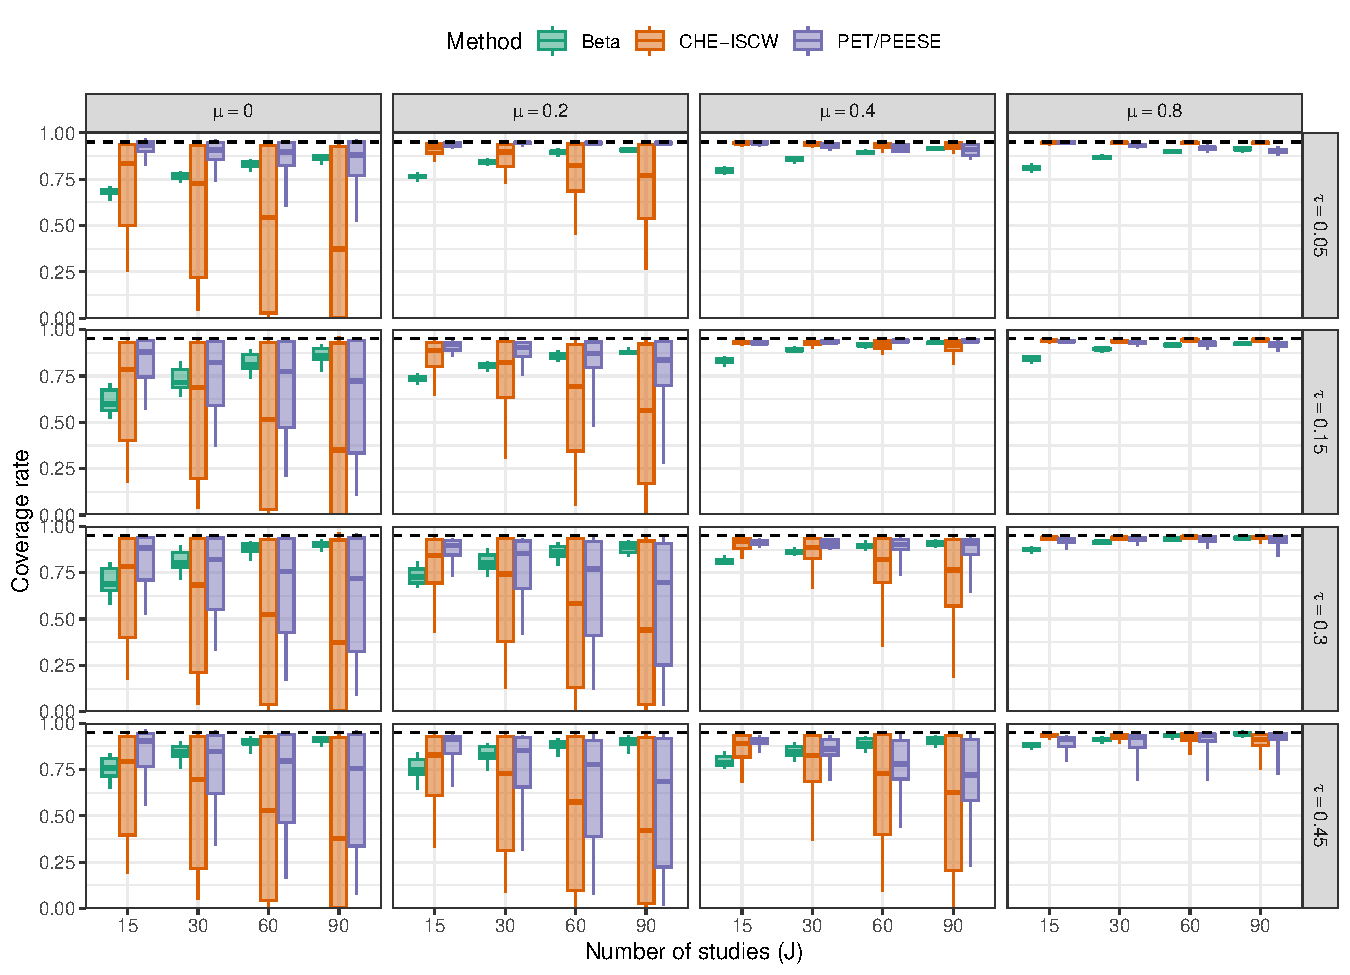
\includegraphics{appendix-simulation-results_files/figure-latex/comparison-coverage-full-main-1} \caption{Coverage levels of confidence intervals for the average effect size based on cluster-robust variance approximations, by method, number of studies, average SMD, and between-study heterogeneity. Dashed lines correspond to the nominal confidence level of 0.95.}\label{fig:comparison-coverage-full-main}
\end{sidewaysfigure}

\section{Beta-Function Selection Model Compared to 3PSM and 4PSM
Step-Function Selection
Models}\label{beta-function-selection-model-compared-to-3psm-and-4psm-step-function-selection-models}

\subsection{\texorpdfstring{Additional simulation results for methods of
estimating the average effect size
\((\mu)\)}{Additional simulation results for methods of estimating the average effect size (\textbackslash mu)}}\label{mu-simulation-results-miss}

\begin{Shaded}
\begin{Highlighting}[]
\NormalTok{mu\_graph\_res\_ci\_miss }\SpecialCharTok{\%\textgreater{}\%}
  \FunctionTok{filter}\NormalTok{(}
\NormalTok{    CI\_type }\SpecialCharTok{\%in\%} \FunctionTok{c}\NormalTok{(}\StringTok{"large{-}sample"}\NormalTok{)}
\NormalTok{  ) }\SpecialCharTok{\%\textgreater{}\%}
  \FunctionTok{ggplot}\NormalTok{(}\FunctionTok{aes}\NormalTok{(}\AttributeTok{x =}\NormalTok{ J, }\AttributeTok{y =}\NormalTok{ coverage, }\AttributeTok{color =}\NormalTok{ method, }\AttributeTok{fill =}\NormalTok{ method)) }\SpecialCharTok{+}
  \FunctionTok{geom\_boxplot}\NormalTok{(}\AttributeTok{alpha =}\NormalTok{ .}\DecValTok{5}\NormalTok{, }\AttributeTok{coef =} \ConstantTok{Inf}\NormalTok{) }\SpecialCharTok{+}
  \FunctionTok{geom\_hline}\NormalTok{(}\AttributeTok{yintercept =} \FloatTok{0.95}\NormalTok{, }\AttributeTok{linetype =} \StringTok{"dashed"}\NormalTok{) }\SpecialCharTok{+}
  \FunctionTok{scale\_y\_continuous}\NormalTok{(}\AttributeTok{limits =} \FunctionTok{c}\NormalTok{(}\ConstantTok{NA}\NormalTok{, }\DecValTok{1}\NormalTok{), }\AttributeTok{expand =} \FunctionTok{expansion}\NormalTok{(}\DecValTok{0}\NormalTok{,}\DecValTok{0}\NormalTok{)) }\SpecialCharTok{+} 
  \FunctionTok{scale\_color\_brewer}\NormalTok{(}\AttributeTok{palette =} \StringTok{"Dark2"}\NormalTok{) }\SpecialCharTok{+}
  \FunctionTok{scale\_fill\_brewer}\NormalTok{(}\AttributeTok{palette =} \StringTok{"Dark2"}\NormalTok{) }\SpecialCharTok{+}
  \FunctionTok{facet\_grid}\NormalTok{(}
\NormalTok{    tau }\SpecialCharTok{\textasciitilde{}}\NormalTok{ mean\_smd, }
    \AttributeTok{labeller =} \FunctionTok{label\_bquote}\NormalTok{(}
      \AttributeTok{rows =}\NormalTok{ tau }\SpecialCharTok{==}\NormalTok{ .(tau),}
      \AttributeTok{cols =}\NormalTok{ mu }\SpecialCharTok{==}\NormalTok{ .(mean\_smd)}
\NormalTok{    ),}
    \AttributeTok{scales =} \StringTok{"free\_y"}
\NormalTok{  ) }\SpecialCharTok{+}
  \FunctionTok{labs}\NormalTok{(}
    \AttributeTok{x =} \StringTok{"Number of studies (J)"}\NormalTok{, }
    \AttributeTok{y =} \StringTok{"Coverage rate"}\NormalTok{, }
    \AttributeTok{color =} \StringTok{"Method"}\NormalTok{,}
    \AttributeTok{fill =} \StringTok{"Method"}
\NormalTok{  ) }\SpecialCharTok{+} 
  \FunctionTok{theme\_bw}\NormalTok{() }\SpecialCharTok{+}
  \FunctionTok{theme}\NormalTok{(}\AttributeTok{legend.position =} \StringTok{"top"}\NormalTok{)}
\end{Highlighting}
\end{Shaded}

\begin{sidewaysfigure}
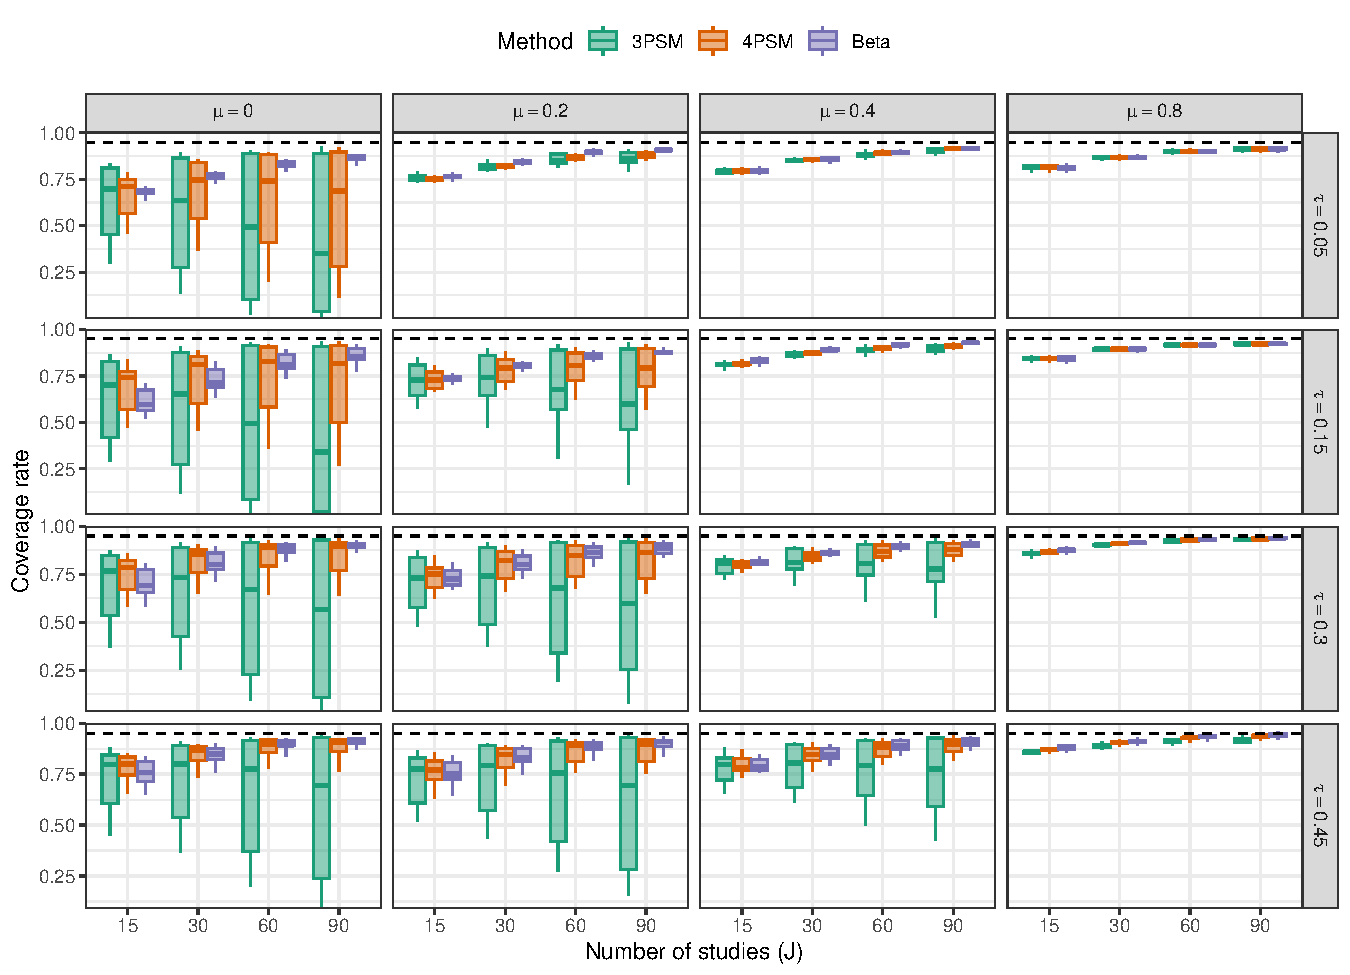
\includegraphics{appendix-simulation-results_files/figure-latex/comparison-coverage-full-miss-1} \caption{Coverage levels of confidence intervals for the average effect size based on cluster-robust variance approximations, by method, number of studies, average SMD, and between-study heterogeneity. Dashed lines correspond to the nominal confidence level of 0.95.}\label{fig:comparison-coverage-full-miss}
\end{sidewaysfigure}

\end{document}
